\clearpage
%%
%% 3 x 2
%%
\begin{table}[htdp]
\caption[Fundamental projectors for matrix (b)]{Fundamental projectors for matrix (b) which has full row rank and represents the overdetermined least squares case. There are no \ns s. The range projectors are identity matrices and the \ns \ projectors are trivial.}
\begin{center}
\begin{tabular}{cc}
%
  $\Axey$ & $\Asyex$\\
%
  $\matrixb  \xtwo   = \ythree$ &
  $\matrixbt \ythree = \xtwo$ \\[20pt]
%
$\Ap =   \AinvL$ & $\paren{\A{*}}^{\sym} \ne \paren{\A{*}}^{-\mathrm{L}} $ \\
$\Ap \ne \AinvR$ & $\paren{\A{*}}^{\sym} =   \paren{\A{*}}^{-\mathrm{R}} $ \\
%
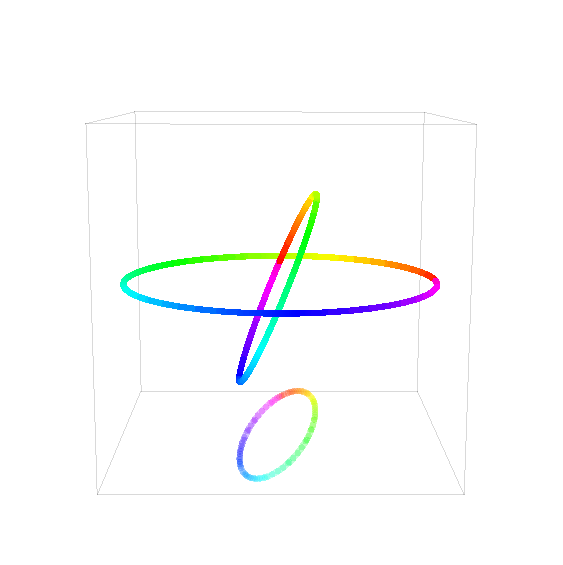
\includegraphics[ width = 2.in ]{images/projectors/a322} &
\includegraphics[ width = 2.in ]{images/projectors/"a322 s"} \\
%
 $\cmplx{2} \quad \mapsto \quad \cmplx{3}$ & 
 $\cmplx{3} \quad \mapsto \quad \cmplx{2}$\\[5pt]\hline
%%
\ \\
 $\pra  = \prab$  & $\pra  = \prabs$ \\
\ \\
 $\pnas = \pnasb$ & $\pnas = \pnasbs$ \\
\ \\
 $\pras = \prasb$ & $\pras = \prasbs$ \\
\ \\
 $\pna  = \pnab$  & $\pna  = \pnabs$
%
\end{tabular}
\end{center}
\label{tab:projector summary:b}
\end{table}

\endinput